\chapter{Lowest Common Ancestor in tempo costante}

\scan{31}

Questo capitolo costruisce, seguendo Harel--Tarjan, una struttura dati che dopo un
pre-processing lineare risponde a ogni query ``qual è il più basso antenato comune di
due nodi?'' in tempo costante. Il percorso è: prima si motiva il problema a
partire dalle applicazioni dei suffix tree, poi lo si risolve sul caso facile
dell'albero binario completo, infine si riporta il caso generale a quello facile
tramite una mappa opportuna.

\section{Perché serve il \texorpdfstring{$\lca$}{lca}: applicazioni dei suffix tree}

I suffix tree hanno \emph{tante} applicazioni: il capitolo~7 di Gusfield ne raccoglie
diciassette, da APL1 ad APL17. Per alcune di esse serve saper calcolare il $\lca$: è
questo il motivo per cui si studia l'algoritmo di Harel--Tarjan.

La più semplice è la ricerca esatta. Dati il testo $T$ e il pattern $P$, si costruisce
$\STree(T)$ e si segue dalla radice il cammino etichettato $P$: il sottoalbero appeso
al punto in cui tale cammino termina ha una dimensione pari al numero di occorrenze di
$P$ in $T$ (le sue foglie \emph{sono} le occorrenze).

\begin{figure}[H]
  \centering
  % Ricerca esatta di P nello STree di T (Gusfield, APL1).
% Il cammino etichettato P scende dalla radice; il sottoalbero appeso al punto
% in cui il cammino termina ha per foglie le occorrenze di P in T.
\begin{tikzpicture}[>=Latex,line join=round]
  \footnotesize

  % ---- sagoma irregolare dello STree(T) ------------------------------------
  \draw[line width=0.7pt,rounded corners=1.2pt]
       (0.40,3.20) -- (0.15,2.78) -- (0.05,2.42) -- (-0.36,2.16) -- (-0.50,1.80)
    -- (-0.96,1.56) -- (-1.14,1.16) -- (-1.70,0.96) -- (-1.94,0.60)
    -- (-2.50,0.44) -- (-2.82,0.16) -- (-3.20,0.00);
  \draw[line width=0.7pt,rounded corners=1.2pt]
       (0.40,3.20) -- (0.72,2.90) -- (0.80,2.50) -- (1.16,2.34) -- (1.30,1.94)
    -- (1.72,1.78) -- (1.86,1.34) -- (2.30,1.14) -- (2.50,0.74)
    -- (2.96,0.50) -- (3.12,0.20) -- (3.30,0.00);

  % ---- livello delle foglie ------------------------------------------------
  \draw[line width=1.1pt] (-3.75,0) -- (3.75,0);
  \node[anchor=east] at (-3.85,0.04) {foglie};

  % ---- sottoalbero delle occorrenze (tratteggiato) -------------------------
  \begin{scope}
    \clip (0.35,1.75) -- (-1.30,0) -- (0.95,0) -- cycle;
    \foreach \k in {-3.4,-3.25,...,0.75}{%
      \draw[gray,line width=0.35pt] (\k,-0.30) -- (\k+2.60,2.30);}
  \end{scope}
  \draw[line width=0.7pt] (-1.30,0) -- (0.35,1.75) -- (0.95,0);

  % ---- cammino etichettato P ----------------------------------------------
  \draw[line width=0.9pt]
       (0.40,3.20) .. controls (0.60,2.92) and (0.16,2.68) .. (0.36,2.42)
                   .. controls (0.56,2.18) and (0.18,1.98) .. (0.35,1.75);
  \node[anchor=west] at (0.50,2.14) {$P$};

  % ---- fine del cammino ----------------------------------------------------
  \fill (0.35,1.75) circle (2.2pt);

  % ---- etichetta della sagoma ---------------------------------------------
  \draw[gray,line width=0.4pt] (-2.12,1.74) -- (-1.08,1.40);
  \node[anchor=east] at (-2.18,1.74) {$\STree(T)$};

  % ---- puntatore alla nota -------------------------------------------------
  \draw[line width=0.6pt,->]
       (-0.20,-0.08) .. controls (0.05,-0.42) and (-0.25,-0.56) .. (0.12,-0.86)
                     .. controls (0.44,-1.10) and (0.70,-0.94) .. (1.00,-1.14);
  \node[anchor=west,align=left] at (1.06,-1.16)
       {tante foglie quante le\\ occorrenze di $P$ in $T$};
\end{tikzpicture}

  \caption{Ricerca di $P$ nello \STree di $T$: il cammino etichettato $P$ scende dalla
    radice fino a un punto dell'albero; il sottoalbero (tratteggiato) appeso a quel
    punto ha tante foglie quante sono le occorrenze di $P$ in $T$.}
  \label{fig:stree-occorrenze}
\end{figure}

\begin{osservazione}
  Il testo viene scandito una volta sola: dopo la costruzione dello \STree, il tempo
  per i pattern successivi è proporzionale alla dimensione del pattern più il numero di
  occorrenze, cioè $\Th(\abs{P}+k)$ per un pattern $P$ con $k$ occorrenze.
\end{osservazione}

Con due testi si procede allo stesso modo, concatenandoli con due terminatori distinti
e non appartenenti all'alfabeto:
\[
  T_1\,\text{\$}\,T_2\,\text{\texteuro}
  \qquad\longrightarrow\qquad
  \STree\bigl(T_1\,\text{\$}\,T_2\,\text{\texteuro}\bigr).
\]
In preprocessing si etichetta ogni foglia a seconda che il suo suffisso contenga o no
il primo separatore: se lo contiene --- forma $\dots\text{\$}\dots\text{\texteuro}$ ---
il suffisso comincia dentro $T_1$; se non lo contiene --- forma
$\dots\text{\texteuro}$, senza \$ --- comincia dentro $T_2$.

\begin{figure}[H]
  \centering
  % Suffix tree generalizzato: STree(T_1 $ T_2 EURO).
% Si scende fino al nodo alpha e si leggono le foglie del suo sottoalbero;
% l'etichetta apposta in preprocessing dice se il suffisso comincia in T_1
% oppure in T_2 (Gusfield, APL4: piu' lunga sottostringa comune).
\begin{tikzpicture}[>=Latex,line join=round]
  \footnotesize

  % ---- sagoma dello STree --------------------------------------------------
  \draw[line width=0.7pt] (0,3.00) -- (-2.20,0) (0,3.00) -- (2.20,0);
  \node[anchor=west] at (0.55,2.72)
       {$\STree\bigl(T_1\,\text{\$}\,T_2\,\text{\texteuro}\bigr)$};
  \draw[gray,line width=0.4pt] (0.50,2.70) -- (0.16,2.62);

  % ---- livello delle foglie, percorso da sinistra a destra -----------------
  \draw[line width=1.0pt,->] (-2.55,0) -- (3.05,0);

  % ---- cammino dalla radice fino ad alpha ----------------------------------
  \draw[line width=0.9pt]
       (0,3.00) .. controls (-0.18,2.78) and (0.04,2.62) .. (-0.14,2.42)
                .. controls (-0.32,2.24) and (-0.12,2.20) .. (-0.30,2.05);
  \fill (-0.30,2.05) circle (2.0pt);
  \node[anchor=west] at (-0.18,2.14) {$\a$};

  % ---- sottoalbero radicato in alpha ---------------------------------------
  \draw[line width=0.7pt] (-0.95,0) -- (-0.30,2.05) -- (0.85,0);

  % ---- foglie del sottoalbero, etichettate in preprocessing ----------------
  \foreach \x/\lab in {-0.78/T_1,-0.26/T_2,0.26/T_2,0.70/T_1}{%
    \fill (\x,0) circle (1.4pt);
    \node[anchor=north,inner sep=2pt,font=\scriptsize] at (\x,-0.06) {$\lab$};}

  \draw[line width=0.5pt,decorate,decoration={brace,amplitude=4pt}]
       (0.90,-0.52) -- (-1.00,-0.52);
  \node[anchor=north] at (-0.05,-0.70) {foglie di $\albero{\a}$};

  % ---- nota ----------------------------------------------------------------
  \node[anchor=west,align=left] at (3.15,0)
       {lettura delle foglie:\\
        suffisso con \$ (forma $\dots\text{\$}\dots\text{\texteuro}$)
        $\Rightarrow$ dentro $T_1$\\
        suffisso senza \$ (forma $\dots\text{\texteuro}$)
        $\Rightarrow$ dentro $T_2$};
\end{tikzpicture}

  \caption{Nello \STree di $T_1\,\text{\$}\,T_2\,\text{\texteuro}$ si scende fino a un nodo $\a$ e si
    leggono le foglie del sottoalbero radicato in $\a$: le etichette apposte in
    preprocessing dicono se la stringa $\a$ occorre in $T_1$, in $T_2$ o in entrambi.}
  \label{fig:stree-generalizzato}
\end{figure}

\section{Il problema e il piano di lavoro}

\begin{definizione}[Lowest common ancestor]\label{def:lca}
  Dato un \emph{albero} $\T$ e due suoi \emph{nodi} $x,y$, si vuole trovare
  $\lca(x,y)$: il nodo $w$ più profondo tale che
  \[
    x,y \in \albero{w},
  \]
  dove $\albero{w}$ denota il sottoalbero di $\T$ radicato in $w$. In particolare
  $x,y\in\albero{\lca(x,y)}$.
\end{definizione}

L'obiettivo è rispondere a ogni query in tempo $\Oh(1)$, dopo un pre-processing che
resti lineare.

\scan{32}

\begin{esempio}
  Lavoreremo con alberi \emph{qualsiasi}, cioè non necessariamente binari né
  bilanciati: si veda l'albero della Figura~\ref{fig:lca-albero-dfs}.
\end{esempio}

\begin{figure}[H]
  \centering
  % Albero generico T con i nodi numerati in dfs-numbering (preordine).
% Accanto ai nodi 1, 2, 5 e' indicato l'intervallo dei numeri DFS del
% sottoalbero radicato in quel nodo: e' sempre un intervallo contiguo.
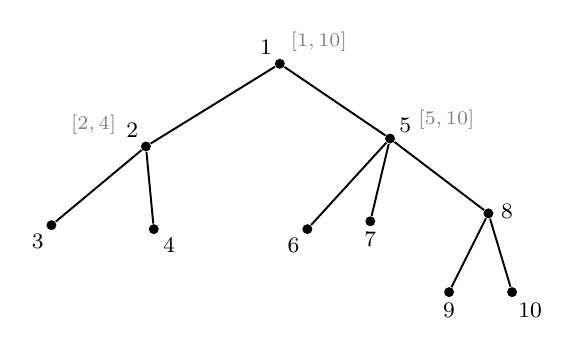
\begin{tikzpicture}[
    nodo/.style={circle,fill,inner sep=0pt,minimum size=3.6pt},
    arco/.style={line width=0.7pt},
    num/.style={inner sep=1.5pt},
    ran/.style={inner sep=1.5pt,text=gray,font=\scriptsize}]
  \footnotesize

  % ---- nodi ----------------------------------------------------------------
  \node[nodo] (n1)  at (3.00, 0.00) {};
  \node[nodo] (n2)  at (1.30,-1.05) {};
  \node[nodo] (n5)  at (4.40,-0.95) {};
  \node[nodo] (n3)  at (0.10,-2.05) {};
  \node[nodo] (n4)  at (1.40,-2.10) {};
  \node[nodo] (n6)  at (3.35,-2.10) {};
  \node[nodo] (n7)  at (4.15,-2.00) {};
  \node[nodo] (n8)  at (5.65,-1.90) {};
  \node[nodo] (n9)  at (5.15,-2.90) {};
  \node[nodo] (n10) at (5.95,-2.90) {};

  % ---- archi ---------------------------------------------------------------
  \draw[arco] (n1) -- (n2)  (n1) -- (n5)
              (n2) -- (n3)  (n2) -- (n4)
              (n5) -- (n6)  (n5) -- (n7)  (n5) -- (n8)
              (n8) -- (n9)  (n8) -- (n10);

  % ---- numeri DFS ----------------------------------------------------------
  \node[num,anchor=south east] at ([shift={(-0.04,0.06)}]n1.center)  {$1$};
  \node[num,anchor=south east] at ([shift={(-0.04,0.06)}]n2.center)  {$2$};
  \node[num,anchor=south west] at ([shift={( 0.06,0.02)}]n5.center)  {$5$};
  \node[num,anchor=north east] at ([shift={(-0.04,-0.06)}]n3.center) {$3$};
  \node[num,anchor=north west] at ([shift={( 0.06,-0.06)}]n4.center) {$4$};
  \node[num,anchor=north east] at ([shift={(-0.04,-0.06)}]n6.center) {$6$};
  \node[num,anchor=north]      at ([shift={( 0.00,-0.08)}]n7.center) {$7$};
  \node[num,anchor=west]       at ([shift={( 0.10,0.02)}]n8.center)  {$8$};
  \node[num,anchor=north]      at ([shift={( 0.00,-0.08)}]n9.center) {$9$};
  \node[num,anchor=north west] at ([shift={( 0.02,-0.08)}]n10.center){$10$};

  % ---- intervalli dei sottoalberi ------------------------------------------
  \node[ran,anchor=south west] at ([shift={( 0.08,0.10)}]n1.center) {$[1,10]$};
  \node[ran,anchor=south east] at ([shift={(-0.32,0.10)}]n2.center) {$[2,4]$};
  \node[ran,anchor=south west] at ([shift={( 0.30,0.06)}]n5.center) {$[5,10]$};
\end{tikzpicture}

  \caption{Un albero generico $\T$ con i nodi numerati secondo la visita in profondità
    (preordine). Accanto ai nodi $1$, $2$ e $5$ è riportato l'intervallo dei numeri DFS
    del rispettivo sottoalbero.}
  \label{fig:lca-albero-dfs}
\end{figure}

Numereremo i nodi in \emph{dfs-numbering}: a ogni nodo si assegna il suo numero
d'ordine nella visita in profondità (preordine). L'assegnazione costa \emph{tempo
lineare} e si può fare mentre si legge l'input. D'ora in avanti identifichiamo ogni
nodo con il proprio numero DFS.

\begin{osservazione}[Proprietà del dfs-numbering]
  I discendenti del nodo $v$ costituiscono un \emph{intervallo}
  \[
    [\,v+1,\ j\,],
  \]
  dove $j-v$ è il numero di tali discendenti. Equivalentemente, i numeri DFS dei nodi
  di $\albero{v}$ formano l'intervallo contiguo
  \[
    [\,v,\ v+\abs{\albero{v}}-1\,],
  \]
  cioè sono assegnati \emph{senza buchi}; in particolare
  $j = v + \abs{\albero{v}} - 1$.
\end{osservazione}

Il problema da risolvere è dunque il calcolo di
\[
  \lca(x,y) \qquad \text{in tempo } \Oh(1),
\]
dove $x$ e $y$ sono i numeri DFS di due nodi di $\T$. Lo strumento tecnico saranno le
\emph{bitmap}: rappresentando l'informazione con stringhe di bit si rendono efficienti
le operazioni di base.

\paragraph{Piano.}
\begin{enumerate}
  \item Risolvo il problema su $\B$, albero binario \emph{completo} (caso facile).
  \item Definisco una mappa
  \[
    I \colon \T \longrightarrow \B, \qquad v \longmapsto I(v),
  \]
  in generale \emph{non} iniettiva.
  \item Uso la mappa e la soluzione in $\Oh(1)$ su $\B$ per risolvere il problema su
  $\T$.
\end{enumerate}

\section{Un modello di calcolo a parole logaritmiche}\label{sec:lca-modello}

\scan{33}

Prima di attaccare il problema devo mettere in discussione il modello di calcolo, cioè
dichiarare esplicitamente quali operazioni considero a costo unitario. In effetti non
lo sto davvero modificando: quelle che seguono sono le assunzioni standard del modello
RAM con parole di lunghezza logaritmica.

Gli assegnamenti
\[
  i \leftarrow i+j, \qquad
  i \leftarrow k, \qquad
  i \leftarrow i/k, \qquad \dots
\]
costano $\Oh(1)$ \emph{se} gli interi coinvolti sono esprimibili mediante $c\log n$
bit, dove $n$ è la dimensione dell'input (per noi: il numero di nodi di $\T$).

Assumo inoltre di poter eseguire in tempo $\Oh(1)$ le seguenti operazioni su array di
$c\log n$ bit, che chiameremo \emph{parole}:
\begin{itemize}
  \item \textsc{and}, \textsc{or}, \textsc{xor} (bit a bit);
  \item \textsc{shift} (\emph{left}/\emph{right}); scriveremo $a \ll s$ e $a \gg s$ per
        lo scorrimento di $a$ di $s$ posizioni verso sinistra e verso destra;
  \item costruzione di una \textsc{mask};
  \item individuazione della posizione dell'1 significativo più a sinistra
        (\emph{leftmost}) o più a destra (\emph{rightmost}).
\end{itemize}

Le posizioni dei bit di una parola sono sempre numerate \emph{da destra} a partire
da~$1$: la posizione $1$ è quella del bit meno significativo. Nella
Sezione~\ref{sec:lca-primitive}, a capitolo concluso, verificheremo che tutte queste
primitive si realizzano davvero in $\Oh(1)$ a partire dalle sole operazioni
aritmetiche, al prezzo di un pre-processing $\Oh(n)$.

\section{Passo 1: il \texorpdfstring{$\lca$}{lca} in un albero binario completo}
\label{sec:lca-passo1}

È il caso facile del piano. Se $\B$ ha $p$ foglie, i suoi livelli contengono
rispettivamente $1, 2, 4, 8, \dots$ nodi e sono dunque in numero logaritmico.

\begin{figure}[H]
  \centering
  % L'albero binario completo B: p foglie, livelli di 1, 2, 4, 8, ... nodi,
% profondita' d = log_2 p.  Sono esplicitati solo i primi tre livelli; i due
% rami esterni (= lati del triangolo) proseguono fino alla linea ondulata
% delle foglie, a indicare che l'albero continua.
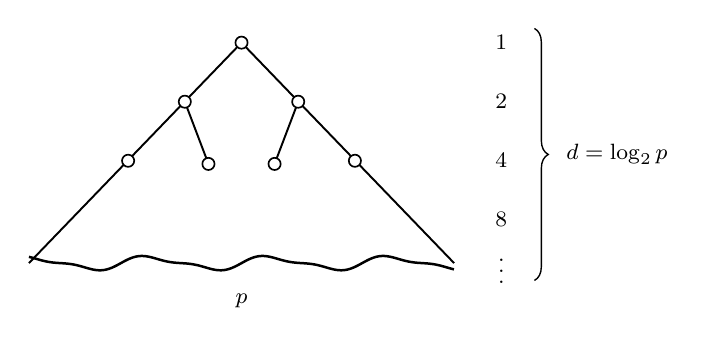
\begin{tikzpicture}[
    nodo/.style={circle,draw,fill=white,line width=0.6pt,
                 inner sep=0pt,minimum size=4.4pt},
    arco/.style={line width=0.7pt}]
  \footnotesize

  % ---- rami esterni: coincidono con i lati del triangolo -------------------
  \draw[arco] (0,2.80) -- (-2.70,0);
  \draw[arco] (0,2.80) -- ( 2.70,0);

  % ---- archi interni dei primi tre livelli ---------------------------------
  \draw[arco] (-0.72,2.05) -- (-0.42,1.26);
  \draw[arco] ( 0.72,2.05) -- ( 0.42,1.26);

  % ---- nodi dei primi tre livelli ------------------------------------------
  \node[nodo] at ( 0.00,2.80) {};
  \node[nodo] at (-0.72,2.05) {};
  \node[nodo] at ( 0.72,2.05) {};
  \node[nodo] at (-1.44,1.30) {};
  \node[nodo] at (-0.42,1.26) {};
  \node[nodo] at ( 0.42,1.26) {};
  \node[nodo] at ( 1.44,1.30) {};

  % ---- livello delle foglie: linea ondulata --------------------------------
  \draw[line width=0.9pt,smooth,samples=160,domain=-2.70:2.70]
        plot (\x,{0.075*sin(\x*235)+0.030*sin(\x*470)});
  \node[anchor=north] at (0,-0.28) {$p$};

  \node at (-1.55,0.50) {$\B$};

  % ---- taglia dei livelli e profondita' ------------------------------------
  \node at (3.30,2.80) {$1$};
  \node at (3.30,2.05) {$2$};
  \node at (3.30,1.30) {$4$};
  \node at (3.30,0.55) {$8$};
  \node at (3.30,0.00) {$\vdots$};
  \draw[line width=0.5pt,decorate,decoration={brace,amplitude=5pt}]
       (3.72,2.98) -- (3.72,-0.22);
  \node[anchor=west] at (4.02,1.38) {$d=\log_2 p$};
\end{tikzpicture}

  \caption{L'albero binario completo $\B$: $p$ foglie, livelli di $1,2,4,8,\dots$ nodi,
    profondità $d=\log_2 p$.}
  \label{fig:b-albero-completo}
\end{figure}

\scan{34}

Riassumendo:
\[
  \B:\qquad
  p \ \text{foglie},\qquad
  2p-1 \ \text{nodi}\ \ (\text{di cui } p-1 \ \text{interni}),\qquad
  d=\log_2 p \ \text{di profondità}.
\]

Ogni nodo $v$ di $\B$ è individuato dal cammino che lo raggiunge a partire dalla
radice: un bit per arco, con la convenzione $0=\text{scendo a sinistra}$,
$1=\text{scendo a destra}$. Per avere codifiche tutte della stessa lunghezza, la
stringa del cammino si completa con un $1$ e con tanti $0$ quanti ne servono: un
generico nodo di $\B$ si codifica così con $d+1$ bit.

\begin{figure}[H]
  \centering
  % path-number-alpha -- codifica di un nodo v di B: i bit del cammino radice->v
% (la stringa alpha), poi il terminatore 1, poi gli 0 di riempimento (quaderno, pag. 33).
\begin{tikzpicture}[
    >={Stealth[length=5pt,width=4pt]},
    font=\small,
    sagoma/.style={semithick,draw=black!65},
    nodo/.style={circle,fill=black,inner sep=0pt,minimum size=3pt},
    parola/.style={thick},
    sep/.style={semithick},
  ]

  %% ------------------------------------------------------------------
  %% Pannello sinistro: la sagoma dell'albero binario completo B
  %% ------------------------------------------------------------------
  \draw[sagoma]
      (-2.20,0.00)
        to[out=68,in=228]  (-1.55,1.05)
        to[out=48,in=252]  (-1.00,1.95)
        to[out=72,in=232]  (-0.50,2.90)   % apice = radice
        to[out=-42,in=152] (-0.02,2.25)
        to[out=-28,in=172] ( 0.52,1.95)
        to[out=-14,in=142] ( 1.20,1.00)
        to[out=-44,in=118] ( 1.90,0.00)
      % base ondulata
        to[out=186,in=-6]  ( 0.75,-0.07)
        to[out=174,in=-6]  (-0.55, 0.06)
        to[out=174,in=-12] (-2.20, 0.00);

  % cammino radice -> v (linea leggermente ondulata)
  \draw[semithick,->]
      (-0.50,2.82)
        to[out=-86,in=94] (-0.42,2.45)
        to[out=-86,in=94] (-0.58,2.10)
        to[out=-86,in=94] (-0.42,1.78)
        to[out=-86,in=98] (-0.50,1.52);
  \node[nodo] (v) at (-0.50,1.44) {};
  \node[right=2pt] at (v) {$v$};
  \node[anchor=west] at (-0.34,2.06) {$\a$};

  %% ------------------------------------------------------------------
  %% Pannello destro: il path number di v come parola di d+1 bit
  %% ------------------------------------------------------------------
  \def\ay{1.10}          % quota della parola
  \def\xa{2.60}          % delimitatore sinistro
  \def\xb{5.40}          % fine della zona alpha
  \def\xc{5.85}          % fine della cella del terminatore
  \def\xd{8.20}          % delimitatore destro

  \node[anchor=west,font=\footnotesize] at (\xa,\ay+0.78) {path number di $v$};

  \draw[parola] (\xa,\ay) -- (\xd,\ay);
  \draw[parola] (\xa,\ay-0.16) -- (\xa,\ay+0.16);
  \draw[parola] (\xd,\ay-0.16) -- (\xd,\ay+0.16);
  \draw[sep]    (\xb,\ay-0.11) -- (\xb,\ay+0.32);
  \draw[sep]    (\xc,\ay-0.11) -- (\xc,\ay+0.32);

  \node[above] at ({0.5*(\xa+\xb)},\ay+0.04) {$\a$};
  \node[above] at ({0.5*(\xb+\xc)},\ay+0.04) {$1$};
  \foreach \i in {0,...,6}{%
    \node[above] at ({\xc+(\i+0.5)*(\xd-\xc)/7},\ay+0.04) {$0$};}

  \draw[decorate,decoration={brace,amplitude=5pt,mirror,raise=2pt},draw=black!65]
      (\xa,\ay-0.16) -- (\xd,\ay-0.16)
      node[midway,below=8pt,font=\footnotesize]{$d+1$ bit};

\end{tikzpicture}

  \caption{Codifica di un nodo $v$ di $\B$: i bit $\a$ del cammino radice--$v$, poi
    un $1$, poi tutti $0$.}
  \label{fig:path-number-alpha}
\end{figure}

\begin{definizione}[Path number]\label{def:path-number}
  Sia $v$ un nodo di $\B$ a profondità $t$ (la radice ha $t=0$) e sia
  $\a=b_1b_2\cdots b_t$ la sequenza di bit che descrive il cammino dalla radice a $v$.
  Il \emph{path number} di $v$ è la parola di $d+1$ bit
  \[
    \underbrace{\ \underbrace{b_1b_2\cdots b_t}_{\a}\ \underbrace{1}_{\text{terminatore}}\ \underbrace{0\cdots 0}_{d-t}\ }_{d+1\ \text{bit}}
  \]
\end{definizione}

\begin{figure}[H]
  \centering
  % lca-b-path-number -- albero binario completo con p=4 foglie e d=2: ogni nodo porta
% il proprio path number in binario e, sotto, in base dieci (quaderno, pag. 34).
\begin{tikzpicture}[
    >={Stealth[length=5pt,width=4pt]},
    font=\small,
    nodo/.style={circle,fill=black,inner sep=0pt,minimum size=3.4pt},
    pn/.style={align=center,inner sep=1.5pt,font=\footnotesize},
    arco/.style={semithick},
  ]

  %% ---- nodi ---------------------------------------------------------
  \node[nodo] (r)  at ( 0.00,2.60) {};   % radice
  \node[nodo] (s)  at (-1.70,1.30) {};   % figlio sinistro
  \node[nodo] (d)  at ( 1.70,1.30) {};   % figlio destro
  \node[nodo] (f1) at (-2.55,0.00) {};
  \node[nodo] (f2) at (-0.85,0.00) {};
  \node[nodo] (f3) at ( 0.85,0.00) {};
  \node[nodo] (f4) at ( 2.55,0.00) {};

  %% ---- archi --------------------------------------------------------
  \draw[arco] (r) -- (s);  \draw[arco] (r) -- (d);
  \draw[arco] (s) -- (f1); \draw[arco] (s) -- (f2);
  \draw[arco] (d) -- (f3); \draw[arco] (d) -- (f4);

  %% ---- path number: binario sopra, valore decimale sotto ------------
  \node[pn,above=3pt]      at (r)  {$100$\\$4$};
  \node[pn,left=4pt]       at (s)  {$010$\\$2$};
  \node[pn,right=4pt]      at (d)  {$110$\\$6$};
  \node[pn,below=3pt]      at (f1) {$001$\\$1$};
  \node[pn,below=3pt]      at (f2) {$011$\\$3$};
  \node[pn,below=3pt]      at (f3) {$101$\\$5$};
  \node[pn,below=3pt]      at (f4) {$111$\\$7$};

  %% ---- annotazione "d+1 bit" sulla codifica della radice ------------
  \node[anchor=west,font=\footnotesize] (bit) at (0.95,3.55) {$d+1$ bit};
  \draw[->,semithick,shorten >=2pt] (bit.west) to[out=180,in=25] (0.28,3.32);

  %% ---- graffa: i tre livelli, profondita' d=2 -----------------------
  \draw[decorate,decoration={brace,amplitude=6pt,raise=2pt},draw=black!65]
      (3.45,2.60) -- (3.45,0.00)
      node[midway,right=9pt,font=\footnotesize]{$d=2$};

\end{tikzpicture}

  \caption{Albero binario completo con $p=4$ foglie, $d=2$: ogni nodo è etichettato con
    il proprio path number (in binario e, sotto, in base dieci).}
  \label{fig:lca-b-path-number}
\end{figure}

Dato $\B$, assegno ad ogni nodo il suo path number e lo manipolo come array di bit: è
un pre-processing lineare. Da qui in avanti identifichiamo ogni nodo di $\B$ con il
proprio path number.

\begin{domanda}
  Come si calcola $\lca_{\B}(x,y)$ in $\B$?
\end{domanda}

\begin{figure}[H]
  \centering
  % lca-b-triangolo -- z = lca_B(x,y): il cammino radice->z e' gamma, e da z i due
% cammini verso x e verso y si separano subito (quaderno, pag. 34).
\begin{tikzpicture}[
    font=\small,
    nodo/.style={circle,fill=black,inner sep=0pt,minimum size=3.4pt},
    livello/.style={semithick,draw=black!55},
    cammino/.style={semithick,rounded corners=2pt},
  ]

  %% ---- la sagoma triangolare di B -----------------------------------
  \coordinate (apice) at (0,4.40);
  \draw[semithick] (-3.00,0) -- (apice) -- (3.00,0) -- cycle;
  \node[font=\footnotesize,text=black!70] at (-2.05,0.55) {$\B$};

  %% ---- i due livelli: quello della radice e quello di z -------------
  \draw[livello] (-1.10,4.40) -- (2.50,4.40);
  \draw[livello] (-1.60,3.35) -- (2.50,3.35);

  % misura della profondita' di z, cioe' della lunghezza di gamma
  \draw[<->,>={Stealth[length=4.5pt,width=3.5pt]},semithick]
      (2.15,4.36) -- (2.15,3.39)
      node[midway,right=2pt,font=\footnotesize]{$\abs{\y}$};

  %% ---- il cammino radice -> z ---------------------------------------
  \node[nodo] (z) at (0,3.35) {};
  \node[right=3pt] at (z) {$z$};
  \draw[line width=1.1pt,-{Stealth[length=6pt,width=5pt]}]
      (0,3.44) -- (0,4.32) node[pos=0.15,left=2pt]{$\y$};

  %% ---- da z i due cammini divergono subito --------------------------
  \draw[cammino]
      (0,3.28) -- (-0.42,2.94) -- (-0.24,2.60) -- (-0.76,2.26)
             -- (-0.58,1.96) -- (-1.20,1.78) -- (-1.55,1.60);
  \draw[cammino]
      (0,3.28) -- ( 0.36,2.94) -- ( 0.18,2.60) -- ( 0.66,2.26)
             -- ( 0.48,1.96) -- ( 1.00,1.78) -- ( 1.25,1.60);

  \node[nodo] (x) at (-1.55,1.60) {};
  \node[nodo] (y) at ( 1.25,1.60) {};
  \node[below left=0pt and 1pt]  at (x) {$x$};
  \node[below right=0pt and 1pt] at (y) {$y$};

\end{tikzpicture}

  \caption{$z=\lca_{\B}(x,y)$ in $\B$: il cammino dalla radice a $z$ è $\y$, e da $z$ i
    due cammini verso $x$ e verso $y$ si separano subito.}
  \label{fig:lca-b-triangolo}
\end{figure}

Siano $x$ e $y$ due nodi distinti di $\B$, nessuno dei due antenato dell'altro, e sia
$z=\lca_{\B}(x,y)$. Detto $\y$ il cammino dalla radice a $z$, i cammini che portano a
$x$ e a $y$ hanno entrambi $\y$ come prefisso e subito dopo divergono: uno prosegue a
sinistra (bit $0$) e l'altro a destra (bit $1$). Se $x<y$, sui path number questo si
legge così:
\[
  \begin{aligned}
    x &: \ \y\ 0\ \ast\cdots\ast\ 1\ 0\cdots 0,\\
    y &: \ \y\ 1\ \ast\cdots\ast\ 1\ 0\cdots 0,\\
    z &: \ \y\ 1\ 0\cdots\cdots\cdots\cdots 0,
  \end{aligned}
\]
dove $\ast\cdots\ast$ sono blocchi di bit arbitrari e ciascun $1$ evidenziato è il
terminatore del rispettivo nodo.

\begin{figure}[H]
  \centering
  % lca-b-array-bit -- i path number di x, y e z=lca_B(x,y) come array di d+1 bit:
% la prima colonna in cui x e y differiscono e' quella del terminatore di z
% (quaderno, pag. 34).
\begin{tikzpicture}[
    >={Stealth[length=4.5pt,width=3.5pt]},
    font=\small,
    parola/.style={thick},
    tacca/.style={semithick},
    etichetta/.style={anchor=east,font=\footnotesize},
    guida/.style={dashed,draw=black!55,thin},
  ]

  %% ---- geometria comune ---------------------------------------------
  \def\xa{0.00}   % delimitatore sinistro
  \def\xb{2.80}   % fine del prefisso comune
  \def\xc{3.30}   % fine della colonna di divergenza
  \def\xd{5.20}   % fine del blocco di bit arbitrari
  \def\xe{5.70}   % fine del terminatore di x e di y
  \def\xf{8.40}   % delimitatore destro
  \def\ra{3.60}   % riga di x
  \def\rb{2.10}   % riga di y
  \def\rc{0.30}   % riga di z

  % la colonna in cui x e y divergono, evidenziata su tutte e tre le righe
  \fill[black!6] (\xb,\rc-0.45) rectangle (\xc,\ra+0.90);

  % una parola: linea spessa con i due delimitatori agli estremi
  \newcommand{\parolabit}[1]{%
    \draw[parola] (\xa,#1) -- (\xf,#1);
    \draw[parola] (\xa,#1-0.16) -- (\xa,#1+0.16);
    \draw[parola] (\xf,#1-0.16) -- (\xf,#1+0.16);}
  % una tacca interna di separazione fra celle
  \newcommand{\tacca}[2]{\draw[tacca] (#1,#2-0.10) -- (#1,#2+0.34);}
  % contenuto di una cella, scritto sopra il segmento
  \newcommand{\cella}[4]{\node[above] at ({0.5*(#1+#2)},#3+0.04) {#4};}

  %% ---- riga 1: path number di x -------------------------------------
  \parolabit{\ra}
  \tacca{\xb}{\ra} \tacca{\xc}{\ra} \tacca{\xd}{\ra} \tacca{\xe}{\ra}
  \cella{\xa}{\xb}{\ra}{$\a$}
  \cella{\xb}{\xc}{\ra}{$0$}
  \cella{\xc}{\xd}{\ra}{$*\cdots*$}
  \cella{\xd}{\xe}{\ra}{$1$}
  \cella{\xe}{\xf}{\ra}{$0\cdots 0$}
  \node[etichetta] at (\xa-0.25,\ra) {p.n.\ di $x$};

  %% ---- riga 2: path number di y -------------------------------------
  \parolabit{\rb}
  \tacca{\xb}{\rb} \tacca{\xc}{\rb} \tacca{\xd}{\rb} \tacca{\xe}{\rb}
  \cella{\xa}{\xb}{\rb}{$\b$}
  \cella{\xb}{\xc}{\rb}{$1$}
  \cella{\xc}{\xd}{\rb}{$*\cdots*$}
  \cella{\xd}{\xe}{\rb}{$1$}
  \cella{\xe}{\xf}{\rb}{$0\cdots 0$}
  \node[etichetta] at (\xa-0.25,\rb) {p.n.\ di $y$};

  %% ---- riga 3: path number di z = lca(x,y) --------------------------
  \parolabit{\rc}
  \tacca{\xb}{\rc} \tacca{\xc}{\rc}
  \cella{\xa}{\xb}{\rc}{$\y$}
  \cella{\xb}{\xc}{\rc}{$1$}
  \cella{\xc}{\xf}{\rc}{$0\cdots\cdots\cdots 0$}
  \node[etichetta] at (\xa-0.25,\rc) {p.n.\ di $z$};

  %% ---- la colonna di divergenza attraversa le tre righe -------------
  \draw[guida] (\xb,\rc-0.45) -- (\xb,\ra+0.90);
  \draw[guida] (\xc,\rc-0.45) -- (\xc,\ra+0.90);
  \node[font=\footnotesize] at ({0.5*(\xb+\xc)},\ra+1.12) {colonna $\ell$};

  %% ---- il prefisso comune di x e y e' esattamente gamma -------------
  \draw[decorate,decoration={brace,amplitude=5pt,mirror,raise=2pt},draw=black!65]
      (\xa,\rb-0.16) -- (\xb,\rb-0.16)
      node[midway,below=8pt,font=\footnotesize] (gm) {$\a=\b=\y$};
  \coordinate (divg) at ({0.5*(\xb+\xc)},\rb-0.32);
  \draw[->,semithick,draw=black!65] (gm.east) to[out=0,in=250] (divg);

\end{tikzpicture}

  \caption{I path number di $x$, $y$ e $z=\lca_{\B}(x,y)$ visti come array di bit. La
    colonna evidenziata è la prima in cui $x$ e $y$ differiscono: lì cade esattamente
    il terminatore di $z$.}
  \label{fig:lca-b-array-bit}
\end{figure}

La prima posizione (da sinistra) in cui i due path number differiscono è dunque
esattamente la posizione del terminatore di $z$: il path number di $z$ si ottiene
ricopiando i bit su cui $x$ e $y$ concordano, mettendo $1$ in quella posizione e $0$ in
tutte le posizioni successive. Sia $\ell$ tale posizione, contata da destra: è la
posizione dell'$1$ più significativo di $x \oplus y$.

\begin{algorithm}[H]
  \caption{$\lca_{\B}$ in un albero binario completo (nessuno dei due nodi antenato
    dell'altro)}
  \label{alg:lca-b}
  \begin{algorithmic}[1]
    \Require i path number $x,y$ di due nodi di $\B$, ciascuno su $d+1$ bit, nessuno
      dei due antenato proprio dell'altro
    \Ensure il path number di $\lca_{\B}(x,y)$
    \State $s \gets x \oplus y$ \Comment{1 \textsc{xor}}
    \If{$s = 0$} \Comment{$x$ e $y$ sono lo stesso nodo}
      \State \Return $x$
    \EndIf
    \State $\ell \gets \textsc{Leftmost1}(s)$ \Comment{1 \emph{leftmost} $1$}
    \State $m \gets \max\{x,y\}$ \Comment{$m$ ha il bit $1$ in posizione $\ell$}
    \State \Return $\bigl(m \gg (\ell-1)\bigr) \ll (\ell-1)$ \Comment{2 \emph{shift}}
  \end{algorithmic}
\end{algorithm}

In forma simmetrica (senza il confronto) lo stesso risultato si scrive
$\bigl((x \gg \ell)\ll \ell\bigr)\ \textsc{or}\ 2^{\ell-1}$. Il conto delle operazioni
è
\[
  1\ \textsc{xor} \ +\ 1\ \textit{leftmost } 1 \ +\ 2\ \textit{shift}
  \qquad\Longrightarrow\qquad \Oh(1) \ \text{nel nuovo modello di calcolo.}
\]

\begin{esercizio}
  Risolvere il caso in cui $x$ è antenato o discendente di $y$.
\end{esercizio}

\begin{osservazione}
  L'esercizio non è un caso di scuola: l'algoritmo di query della
  Sezione~\ref{sec:lca-query} invocherà $\lca_{\B}$ su $I(x)$ e $I(y)$, e nulla
  impedisce che quei due path number siano uno antenato dell'altro in $\B$; accade
  anzi spesso che coincidano, cioè che $I(x)=I(y)$, ed è per questo che
  l'Algoritmo~\ref{alg:lca-b} tratta a parte il caso $s=0$. La versione generale resta
  comunque $\Oh(1)$: si verifica che la posizione da cui ripartire non è $\ell$, ma il
  massimo fra $\ell$ e le posizioni dell'$1$ \emph{meno} significativo di $x$ e di $y$.
\end{osservazione}

\section{Passo 2: la mappa \texorpdfstring{$I\colon\T\to\B$}{I : T -> B}}
\label{sec:lca-passo2}

\scan{35}

Il secondo passo consiste nel mandare l'albero generico $\T$ dentro l'albero binario
completo $\B$, per poter riusare l'algoritmo del passo~1. La mappa che costruiremo,
\[
  I \colon \T \longrightarrow \B, \qquad v \longmapsto I(v),
\]
\emph{non} sarà iniettiva.

\begin{osservazione}
  $\B$ non verrà davvero costruito: resta un albero \emph{implicito}. I suoi nodi
  \emph{sono} i loro path number, e ogni operazione su di essi è un'operazione su
  parole di bit.
\end{osservazione}

Identifico i nodi di $\T$ con i \emph{dfs-numeri} loro assegnati in una fase di
pre-processing, cioè con i numeri prodotti da una visita in profondità: una fase che
resta sempre lineare.

\begin{figure}[H]
  \centering
  % L'albero generico T con i dfs-numeri e la loro codifica binaria su 4 bit.
\begin{tikzpicture}[
    x=1.22cm, y=1.20cm,
    nodo/.style={circle, fill=black, inner sep=0pt, minimum size=3.4pt},
    ramo/.style={line width=0.5pt, black!70},
    et/.style={align=center, inner sep=1.2pt, font=\footnotesize}
  ]

  % --- posizioni dei nodi (dfs-numbering in preordine) ---
  \coordinate (v1)  at ( 0.00,  0.00);
  \coordinate (v2)  at (-1.50, -1.20);
  \coordinate (v5)  at ( 2.40, -1.00);
  \coordinate (v3)  at (-2.50, -2.40);
  \coordinate (v4)  at (-1.10, -2.40);
  \coordinate (v6)  at ( 1.20, -2.40);
  \coordinate (v7)  at ( 2.45, -2.40);
  \coordinate (v8)  at ( 3.90, -2.20);
  \coordinate (v9)  at ( 3.45, -3.45);
  \coordinate (v10) at ( 5.00, -3.20);

  % --- archi ---
  \draw[ramo] (v1) -- (v2) (v1) -- (v5)
              (v2) -- (v3) (v2) -- (v4)
              (v5) -- (v6) (v5) -- (v7) (v5) -- (v8)
              (v8) -- (v9) (v8) -- (v10);

  % --- nodi ---
  \foreach \n in {1,2,3,4,5,6,7,8,9,10} { \node[nodo] at (v\n) {}; }

  % --- etichette: dfs-numero (interno) e codifica binaria (esterna) ---
  \node[et, anchor=south]      at ($(v1)+(0,0.10)$)      {$0001$\\$1$};
  \node[et, anchor=south east] at ($(v2)+(-0.08,0.02)$)  {$0010$\\$2$};
  \node[et, anchor=south west] at ($(v5)+(0.10,0.02)$)   {$0101$\\$5$};
  \node[et, anchor=north]      at ($(v3)+(0,-0.10)$)     {$3$\\$0011$};
  \node[et, anchor=north]      at ($(v4)+(0,-0.10)$)     {$4$\\$0100$};
  \node[et, anchor=north]      at ($(v6)+(0,-0.10)$)     {$6$\\$0110$};
  \node[et, anchor=north]      at ($(v7)+(0,-0.10)$)     {$7$\\$0111$};
  \node[et, anchor=south west] at ($(v8)+(0.08,0.10)$)   {$8$\\$1000$};
  \node[et, anchor=north]      at ($(v9)+(0,-0.10)$)     {$9$\\$1001$};
  \node[et, anchor=north]      at ($(v10)+(0,-0.10)$)    {$10$\\$1010$};

\end{tikzpicture}

  \caption{L'albero generico $\T$ con i dfs-numeri e la loro codifica binaria su
    $\lfloor\log_2 n\rfloor+1 = 4$ bit ($n=10$ nodi).}
  \label{fig:lca-albero-I}
\end{figure}

\begin{definizione}[la funzione $h$]\label{def:h}
  Per ogni numero $k$, $h(k)$ è la posizione del suo \emph{rightmost} $1$, cioè la
  posizione, contata da destra a partire da $1$, del bit $1$ meno significativo nella
  rappresentazione binaria di $k$.
\end{definizione}

\begin{osservazione}
  $h(k)$ è l'\emph{altezza di $k$ in $\B$}: è l'altezza del nodo di $\B$ che ha $k$
  come path number, dove l'altezza di un nodo è il numero di nodi sul cammino che lo
  congiunge a una foglia. Infatti un nodo a profondità $t$ ha path number
  $b_1\cdots b_t\,1\,0^{\,d-t}$, il cui $1$ meno significativo sta in posizione
  $d-t+1$, che è esattamente il numero di nodi sul cammino da esso a una foglia.
  Inoltre $h(k)$ si calcola in $\Oh(1)$ con la primitiva \textsc{rightmost}.
\end{osservazione}

\begin{definizione}[la mappa $I$]\label{def:mappa-I}
  Dato $v \in \T$, indico con $I(v)$ il nodo $w \in \albero{v}$ tale che $h(w)$ è
  massimo.
\end{definizione}

\begin{osservazione}
  Due avvertenze sulla definizione. Primo: $h(w)$ è la funzione aritmetica appena
  definita, applicata al \emph{dfs-numero} di $w$; non è l'altezza di $w$ dentro $\T$.
  Secondo: $I(v)$ è, letteralmente, un nodo di $\T$; lo si identifica con il nodo di
  $\B$ che ha $I(v)$ come path number, ed è in questo senso che $I$ è una mappa da
  $\T$ a $\B$.
\end{osservazione}

\begin{esempio}\label{ex:I-esempio}
  Nell'albero della Figura~\ref{fig:lca-albero-I}
  \[
    I(1) = I(5) = I(8) = 8 .
  \]
  Infatti $h(8) = h(1000) = 4$ è il massimo valore di $h$ su tutto l'albero, e il nodo
  $8$ appartiene ai sottoalberi radicati in $1$, in $5$ e in $8$.
\end{esempio}

\begin{osservazione}
  $I(v) = v$ per ogni foglia $v$: il sottoalbero di una foglia è la foglia stessa.
\end{osservazione}

\begin{osservazione}
  $h(I(v))$ non decresce muovendosi verso la radice: se $u$ è un antenato di $v$ allora
  $\albero{v} \subseteq \albero{u}$, e quindi il massimo di $h$ su $\albero{u}$ è
  almeno quello su $\albero{v}$, cioè $h(I(u)) \ge h(I(v))$. Detto altrimenti,
  l'immagine di $v$ sale in $\B$ man mano che $v$ sale in $\T$.
\end{osservazione}

La mappa $I \colon \T \to \B$ definisce implicitamente una relazione di equivalenza sui
nodi di $\T$,
\[
  u \sim v \quad\iff\quad I(u) = I(v),
\]
le cui classi sono i gruppi di nodi evidenziati nella
Figura~\ref{fig:lca-run-map}.

\begin{domanda}
  La funzione $I$ è ben definita?
\end{domanda}

\subsection{Buona definizione e run}

\scan{36}

Perché la mappa $I$ sia ben definita occorre che per ogni elemento del dominio
$v \in \T$ ci sia \emph{uno e un solo} elemento $w \in \B$ tale che $I(v) = w$. Un tale
$w$ esiste sempre --- $\albero{v}$ è finito e non vuoto, dunque il massimo di $h$ su
$\albero{v}$ viene certamente raggiunto: c'è sempre almeno un elemento del codominio.
Resta perciò da provare che non ne possono essere \emph{due}.

\begin{proposizione}[buona definizione di $I$]\label{prop:I-ben-definita}
  Per ogni nodo $v \in \T$ esiste un \emph{unico} nodo $w \in \albero{v}$ tale che
  \[
    h(w) \;=\; \max_{q \in \albero{v}} h(q).
  \]
\end{proposizione}

\begin{dimostrazione}
  Per assurdo, assumiamo che esistano $u, w \in \albero{v}$ con $u \neq w$ e
  \[
    h(u) \;=\; h(w) \;\geq\; h(q) \qquad \text{per ogni } q \in \albero{v}.
  \]
  Poniamo $i \defeq h(u) = h(w)$ e supponiamo, senza perdita di generalità, $w < u$ (il
  confronto è fra i numeri DFS). Sia $k$ la posizione del bit più significativo in cui
  $u$ e $w$ differiscono: poiché $w < u$, in posizione $k$ il numero $u$ ha $1$ e il
  numero $w$ ha $0$. Inoltre $k > i$: infatti $u$ e $w$ hanno entrambi l'$1$ meno
  significativo in posizione $i$ e tutti $0$ nelle posizioni $< i$, quindi non possono
  differire in una posizione $\leq i$.

  Costruiamo allora il numero $N$ che coincide con $u$ e con $w$ in tutte le posizioni
  $> k$, vale $1$ in posizione $k$ ed è nullo in tutte le posizioni $< k$:
  \[
    \begin{array}{c||c|c|c|c|c}
      & \text{pos.} > k & k & k-1,\dots,i+1 & i & i-1,\dots,1\\
      \hline\hline
      u & \a & 1 & \cdots      & 1 & 0\cdots 0\\
      \hline
      w & \a & 0 & \cdots      & 1 & 0\cdots 0\\
      \hline
      N & \a & 1 & 0\cdots 0   & 0 & 0\cdots 0
    \end{array}
  \]
  dove $\a$ denota il prefisso comune (i bit dalla posizione più significativa fino
  alla posizione $k+1$, uguali in $u$, $w$ e $N$) e i puntini nelle righe di $u$ e $w$
  stanno per bit arbitrari.

  È ovvio che
  \[
    w \;<\; N \;<\; u :
  \]
  $N$ e $w$ coincidono sopra la posizione $k$, dove però $N$ ha $1$ e $w$ ha $0$, da
  cui $N > w$; $N$ e $u$ coincidono da sinistra fino a $k$ incluso, ma sotto $k$ il
  numero $N$ ha solo zeri mentre $u$ ha un $1$ in posizione $i < k$, da cui $N < u$.

  Per la proprietà del dfs-numbering (i numeri dei nodi di
  $\albero{v}$ formano un intervallo contiguo, cioè sono assegnati \emph{senza buchi}),
  da $w, u \in \albero{v}$ e $w < N < u$ segue
  \[
    N \in \albero{v}.
  \]
  Ma per costruzione l'$1$ meno significativo di $N$ sta in posizione $k$, cioè
  $h(N) = k > i$, e quindi
  \[
    h(N) \;>\; h(u) \;=\; h(w),
  \]
  contro la massimalità di $h(u) = h(w)$ su $\albero{v}$: assurdo.
\end{dimostrazione}

\begin{figure}[H]
  \centering
  % A sinistra l'albero generico T con i sette run; a destra l'albero binario
% completo B con i sette nodi immagine marcati.
\begin{tikzpicture}[
    x=1cm, y=1cm,
    nodo/.style={circle, fill=black, inner sep=0pt, minimum size=3.2pt},
    nodog/.style={circle, fill=black!45, inner sep=0pt, minimum size=2.6pt},
    anello/.style={circle, draw=black, line width=0.5pt, inner sep=0pt,
                   minimum size=7pt},
    ramo/.style={line width=0.5pt, black!70},
    ramog/.style={line width=0.45pt, black!45},
    run/.style={dash pattern=on 2pt off 1.6pt, line width=0.5pt, black!60},
    et/.style={align=center, inner sep=1pt, font=\scriptsize},
    etg/.style={et, text=black!50}
  ]

  %% ================= PANNELLO SINISTRO: albero T =================
  \coordinate (t1)  at (1.90,  0.00);
  \coordinate (t2)  at (0.85, -0.90);
  \coordinate (t5)  at (2.85, -0.90);
  \coordinate (t3)  at (-0.05, -1.80);
  \coordinate (t4)  at (0.85, -1.80);
  \coordinate (t6)  at (2.10, -1.80);
  \coordinate (t7)  at (2.95, -1.80);
  \coordinate (t8)  at (3.80, -1.80);
  \coordinate (t9)  at (3.58, -2.70);
  \coordinate (t10) at (4.40, -2.70);

  \draw[ramo] (t1) -- (t2) (t1) -- (t5)
              (t2) -- (t3) (t2) -- (t4)
              (t5) -- (t6) (t5) -- (t7) (t5) -- (t8)
              (t8) -- (t9) (t8) -- (t10);

  \foreach \n in {1,2,3,4,5,6,7,8,9,10} { \node[nodo] at (t\n) {}; }

  % --- i sette run ---
  \begin{scope}[rotate around={-43.45:(2.85,-0.90)}]
    \draw[run] (2.85,-0.90) ellipse [x radius=1.57, y radius=0.27];
  \end{scope}
  \draw[run] (0.85,-1.35) ellipse [x radius=0.25, y radius=0.70];
  \foreach \n in {3,6,7,9,10} { \draw[run] (t\n) circle [radius=0.22]; }

  % --- etichette: dfs-numero e path number su 4 bit ---
  \node[et, anchor=south]      at (1.90,  0.28) {$0001$\\$1$};
  \node[et, anchor=south east] at (0.62, -0.72) {$0010$\\$2$};
  \node[et, anchor=south west] at (3.02, -0.55) {$0101$\\$5$};
  \node[et, anchor=north]      at (-0.05, -2.10) {$3$\\$0011$};
  \node[et, anchor=north]      at (0.85, -2.10) {$4$\\$0100$};
  \node[et, anchor=north]      at (2.10, -2.10) {$6$\\$0110$};
  \node[et, anchor=north]      at (2.95, -2.10) {$7$\\$0111$};
  \node[et, anchor=south west] at (4.00, -1.50) {$8=1000$};
  \node[et, anchor=north]      at (3.58, -2.96) {$9$\\$1001$};
  \node[et, anchor=north]      at (4.40, -2.96) {$10$\\$1010$};

  \node[anchor=west, font=\small] at (-0.15, 0.40) {$\T$};

  %% ================= PANNELLO DESTRO: albero binario completo B =========
  \coordinate (b1000) at (8.40,  0.00);
  \coordinate (b0100) at (7.00, -0.85);
  \coordinate (b1100) at (9.80, -0.85);
  \coordinate (b0010) at (6.30, -1.70);
  \coordinate (b0110) at (7.70, -1.70);
  \coordinate (b1010) at (9.10, -1.70);
  \coordinate (b1110) at (10.50,-1.70);
  \coordinate (b0001) at (5.95, -2.55);
  \coordinate (b0011) at (6.65, -2.55);
  \coordinate (b0101) at (7.35, -2.55);
  \coordinate (b0111) at (8.05, -2.55);
  \coordinate (b1001) at (8.75, -2.55);
  \coordinate (b1011) at (9.45, -2.55);
  \coordinate (b1101) at (10.15,-2.55);
  \coordinate (b1111) at (10.85,-2.55);

  \draw[ramog] (b1000) -- (b0100) (b1000) -- (b1100)
               (b0100) -- (b0010) (b0100) -- (b0110)
               (b1100) -- (b1010) (b1100) -- (b1110)
               (b0010) -- (b0001) (b0010) -- (b0011)
               (b0110) -- (b0101) (b0110) -- (b0111)
               (b1010) -- (b1001) (b1010) -- (b1011)
               (b1110) -- (b1101) (b1110) -- (b1111);

  % nodi non marcati
  \foreach \n in {0010,0101,1100,1110,0001,1011,1101,1111}
    { \node[nodog] at (b\n) {}; }
  % nodi marcati: immagine di un run di T
  \foreach \n in {1000,0100,0110,1010,0011,0111,1001}
    { \node[anello] at (b\n) {}; \node[nodo] at (b\n) {}; }

  \node[et, anchor=south]      at (8.40,  0.14) {$1000$};
  \node[et, anchor=south east] at (6.88, -0.74) {$0100$};
  \node[etg,anchor=south west] at (9.92, -0.74) {$1100$};
  \node[et, anchor=north east] at (7.52, -1.82) {$0110$};
  \node[et, anchor=south east] at (8.96, -1.60) {$1010$};
  \node[et, anchor=north]      at (6.65, -2.70) {$0011$};
  \node[et, anchor=north]      at (8.05, -2.70) {$0111$};
  \node[et, anchor=north]      at (8.75, -2.70) {$1001$};

  \node[anchor=west, font=\small] at (5.85, 0.40) {$\B$};

  %% ================= la mappa I =================
  \draw[-{Latex[length=4pt,width=3.2pt]}, dashed, line width=0.6pt, black!60]
        (5.08,-2.00) -- (5.86,-2.00)
        node[midway, above=1pt, font=\scriptsize, text=black] {$I$};

\end{tikzpicture}

  \caption{A sinistra l'albero generico $\T$ con la numerazione DFS (in binario su $4$
    bit) e i sette \emph{run} evidenziati; a destra l'albero binario completo $\B$, in
    cui sono marcati i nodi che sono immagine di qualche nodo di $\T$. La mappa $I$
    collassa ogni run in un unico nodo di $\B$.}
  \label{fig:lca-run-map}
\end{figure}

La mappa $I$ definisce dei \emph{run} di nodi in $\T$.

\begin{definizione}[run]\label{def:run}
  Un \emph{run} è una collezione massimale di nodi di $\T$ mappati nello stesso $I(v)$;
  equivalentemente, è una classe di equivalenza della relazione
  $u \sim v \iff I(u) = I(v)$.
\end{definizione}

\begin{osservazione}
  Ogni run è un \emph{cammino verticale} di $\T$. Anzitutto due nodi dello stesso run
  sono confrontabili: se $I(u)=I(v)$ allora il nodo $I(u)$ appartiene sia ad
  $\albero{u}$ sia ad $\albero{v}$, e due sottoalberi che hanno un nodo in comune sono
  confrontabili per inclusione, cioè uno fra $u$ e $v$ è antenato dell'altro. Il run è
  inoltre \emph{contiguo}: se $u$ è antenato di $v$ e $I(u)=I(v)=w$, ogni nodo $m$ del
  cammino da $u$ a $v$ soddisfa $\albero{v}\subseteq\albero{m}\subseteq\albero{u}$,
  quindi il massimo di $h$ su $\albero{m}$ è compreso fra quello su $\albero{v}$ e
  quello su $\albero{u}$, che valgono entrambi $h(w)$; poiché $w\in\albero{v}\subseteq
  \albero{m}$, quel massimo è realizzato proprio da $w$ e dunque $I(m)=w$. Una catena
  contigua di nodi è un cammino verticale, e lungo un cammino verticale «più vicino
  alla radice» equivale a «numero DFS più piccolo».
\end{osservazione}

\section{Passo 3: il pre-processing}\label{sec:lca-preprocessing}

\scan{37}

Eseguiamo un pre-processing lineare in cui, per ogni nodo $v$ di $\T$, calcoliamo
\[
  \begin{cases}
    I(v),\\[2pt]
    L(v) = \text{il \emph{leader} del suo run},\\[2pt]
    A_v = \text{un array ausiliario}.
  \end{cases}
\]

\begin{osservazione}
  Il nodo di $\albero{v}$ su cui $h$ è massimo --- cioè $I(v)$ --- è il nodo più
  \emph{basso} del run: è il \emph{bottom} del run.
\end{osservazione}

\begin{definizione}[leader di un run]\label{def:leader}
  Definisco \emph{leader} (o \emph{head}) di un run il nodo più \emph{alto} del run,
  cioè quello più vicino alla radice di $\T$.
\end{definizione}

\paragraph{Pre-processing.}
\begin{enumerate}
  \item \textsc{dfs} di $\T$ $\longrightarrow$ computo il \emph{dfs-numbering} e $h(v)$
        per ogni $v$.

  \item Usando $h(\cdot)$ determino $I(\cdot)$ per ogni $v$ mediante una visita
        \emph{bottom-up}. Nella stessa visita determino il leader di ogni run (la
        tabella dei leader è indicizzata dai valori di $I$: $L(v)=L(I(v))$). Ora, per
        ogni $v$, leggo $I(v)$ e $L(v)$ in tempo $\Oh(1)$.

  \item Costruisco $\B$, l'albero binario completo di profondità $d$, dove $d+1$ è il
        numero di bit necessari a scrivere i numeri DFS di $\T$, cioè
        $d+1=\lfloor\log_2 n\rfloor+1$. I path number dei nodi di $\B$ sono allora
        tutte e sole le parole non nulle di $d+1$ bit, ossia gli interi da $1$ a
        $2^{d+1}-1\ge n$: le due numerazioni si possono identificare. (Se $n$ non è una
        potenza di $2$ si ha $d+1=\lceil \log_2 n\rceil$; se lo è, serve un bit in più.)

  \item Per ogni $v$ costruisco $A_v$, array di $d+1$ bit definito da
        \[
          A_v[i] = 1 \iff \exists\, w \text{ antenato di } v \text{ in } \T
          \text{ tale che } h\bigl(I(w)\bigr) = i ,
        \]
        con la convenzione che $v$ è antenato di se stesso.
\end{enumerate}

\begin{figure}[H]
  \centering
  % Il vettore di bit A_v: un array di d+1 = floor(log_2 n)+1 bit; i bit sono numerati da
% destra a partire da 1.
\begin{tikzpicture}[
    x=1cm, y=1cm,
    bordo/.style={line width=0.7pt},
    sep/.style={line width=0.5pt},
    onda/.style={decorate, decoration={snake, amplitude=2pt, segment length=22pt},
                 line width=0.5pt}
  ]

  % --- la parola ---
  \def\hh{0.72}
  \draw[bordo] (0,0) rectangle (7,\hh);

  % separatori fra le celle
  \foreach \x in {3.5, 4.2, 4.9, 5.6, 6.3} { \draw[sep] (\x,0) -- (\x,\hh); }

  % contenuto delle celle: ~ = bit qualsiasi
  \draw[onda] (0.30,0.36) -- (3.20,0.36);
  \draw[onda, decoration={snake, amplitude=1.6pt, segment length=13pt}]
        (4.31,0.36) -- (4.79,0.36);
  \node[font=\small] at (3.85,0.36) {$1$};
  \node[font=\small] at (5.25,0.36) {$1$};
  \node[font=\small] at (5.95,0.36) {$0$};
  \node[font=\small] at (6.65,0.36) {$0$};

  % --- etichetta del vettore ---
  \node[anchor=east, font=\small] at (-0.45,0.36) {$A_v$};

  % --- la posizione puntata ---
  \node[anchor=south, font=\footnotesize] at (3.85,\hh+0.06) {$i$};

  \draw[-{Latex[length=4pt,width=3.4pt]}, line width=0.6pt]
        (3.85,-0.06) -- (3.85,-0.80);

  \node[anchor=north, align=center, font=\small] at (3.85,-0.92)
       {significa che esiste $w$ antenato di $v$\\
        che mappa ad altezza $i$ in $\B$};

\end{tikzpicture}

  \caption{Il vettore di bit $A_v$: un $1$ in posizione $i$ significa che esiste un
    antenato $w$ di $v$ che viene mappato ad altezza $i$ in $\B$.}
  \label{fig:av-bitvector}
\end{figure}

\begin{osservazione}
  Tutti e quattro i passi costano $\Oh(n)$: in particolare $A_v$ si calcola con una
  visita top-down ponendo
  \[
    A_v = A_{\mathrm{padre}(v)} \ \textsc{or}\ 2^{\,h(I(v))-1},
  \]
  cioè con un'operazione $\Oh(1)$ per nodo. Il pre-processing complessivo è dunque
  lineare.
\end{osservazione}

\begin{osservazione}
  Il bit $1$ più a destra di $A_v$ sta in posizione $h(I(v))$: per
  la monotonia di $h\circ I$ ogni antenato $u$ di $v$ ha $h(I(u)) \ge h(I(v))$, e la
  posizione $h(I(v))$ è occupata da $v$ stesso.
\end{osservazione}

\section{Rispondere alle query in tempo costante}\label{sec:lca-query}

\scan{38}

Restano due cose da fare: mostrare che \emph{$I$ mantiene la relazione
antenato/discendente}, e scrivere un algoritmo che, usando $I$, $L$ e gli $A_v$,
risponda a $\lca(x,y)$ in $\Oh(1)$ nel modello di calcolo fissato.

\begin{lemma}[la mappa $I$ rispetta la relazione antenato/discendente]\label{lem:lca-I-ant}
  Siano $x$ e $z$ nodi di $\T$. Allora
  \[
    x\in\albero{z}
    \quad\Longrightarrow\quad
    I(x)\in\B\bigl(I(z)\bigr),
  \]
  dove $\albero{z}$ è il sottoalbero di $\T$ radicato in $z$ e $\B(w)$ è il
  sottoalbero di $\B$ radicato in $w$.
\end{lemma}

\begin{dimostrazione*}
  Distinguiamo due casi.
  \begin{itemize}
    \item Se $I(x)=I(z)$, allora $I(x)=I(z)\in\B\bigl(I(z)\bigr)$ e la tesi è
          immediata: $x$ e $z$ stanno sullo stesso run.

    \item Altrimenti $h\bigl(I(z)\bigr)>h\bigl(I(x)\bigr)$: da
          $\albero{x}\subseteq\albero{z}$ segue
          $h\bigl(I(x)\bigr)\le h\bigl(I(z)\bigr)$ per massimalità, e l'uguaglianza è
          esclusa dall'unicità del nodo che realizza il massimo di $h$ su $\albero{z}$
          (Proposizione~\ref{prop:I-ben-definita}).

          Sia $h\bigl(I(z)\bigr)=i$: i bit a sinistra della posizione $i$ in $I(x)$
          devono essere uguali a quelli a sinistra di $i$ in $I(z)$.

          Da qui segue che $I(x)$ è discendente di $I(z)$ in $\B$. Il sottoalbero di
          $\B$ radicato in un nodo $w$ è infatti esattamente l'insieme dei path number
          che coincidono con $w$ in tutti i bit a sinistra della posizione $h(w)$
          \emph{e} hanno l'$1$ meno significativo in posizione $\le h(w)$: senza
          quest'ultima clausola vi rientrerebbero anche gli antenati di $w$ (per
          esempio, con $d=2$, la radice $100$ coincide con $w=110$ nell'unico bit a
          sinistra di $h(w)=2$). Per $I(x)$ valgono entrambe le condizioni: la prima
          per quanto appena osservato, la seconda perché in questo caso
          $h\bigl(I(x)\bigr)<i$.
  \end{itemize}
\end{dimostrazione*}

\begin{esercizio}[il passaggio lasciato in sospeso]\label{ex:lca-bit-sx}
  Nelle ipotesi del Lemma~\ref{lem:lca-I-ant} e posto $i=h\bigl(I(z)\bigr)$, dimostrare
  che i bit di $I(x)$ a sinistra della posizione $i$ coincidono con quelli di $I(z)$.
\end{esercizio}

\emph{Traccia.} $I(x)$ e $I(z)$ sono numeri DFS di nodi di $\albero{z}$, che per la
proprietà DFS formano un intervallo contiguo. Se i due numeri differissero in qualche
posizione $k>i$, si prenda la più significativa di tali posizioni e si ponga
\[
  N=\bigl(\text{bit comuni a sinistra di }k\bigr)\,\Vert\,1\,\Vert\,0\cdots 0 ,
\]
dove $\Vert$ denota la giustapposizione di stringhe di bit. Allora $\min\{I(x),I(z)\}<N<\max\{I(x),I(z)\}$ e $h(N)=k>i$: dunque $N$ sarebbe il
numero di un nodo di $\albero{z}$ con $h$ maggiore di $h\bigl(I(z)\bigr)$, contro la
definizione di $I(z)$.

\bigskip

I due teoremi che seguono sono il cuore dell'algoritmo di query: il primo dice che
basta conoscere \emph{l'altezza in $\B$} dell'immagine del $\lca$ per ricostruire il
$\lca$ stesso, il secondo dice come si calcola quell'altezza.

\begin{teorema}[determinare $z$ noto $h(I(z))$]\label{thm:lca-teo1}
  Sia $z=\lca(x,y)$. Se conosco $h\bigl(I(z)\bigr)$, allora determino $z$ in $\Oh(1)$.
\end{teorema}

\begin{teorema}[determinare $h(I(z))$ da $A_x$ e $A_y$]\label{thm:lca-teo2}
  Sia $z=\lca(x,y)$ e sia
  \[
    j=\min\Bigl\{\,k\ :\ k\ \ge\ h\bigl(\lca_{\B}(I(x),I(y))\bigr)
    \ \wedge\ A_x[k]=A_y[k]=1\,\Bigr\}.
  \]
  Allora $j=h\bigl(I(z)\bigr)$.
\end{teorema}

\emph{Traccia della dimostrazione del Teorema~\ref{thm:lca-teo2}.} Poniamo
$b=\lca_{\B}(I(x),I(y))$. Da un lato $z$ è antenato comune di $x$ e $y$, quindi
$A_x\bigl[h(I(z))\bigr]=A_y\bigl[h(I(z))\bigr]=1$; inoltre, per il
Lemma~\ref{lem:lca-I-ant}, $I(z)$ è antenato in $\B$ sia di $I(x)$ sia di $I(y)$, dunque
è antenato di $b$ e $h(I(z))\ge h(b)$: il valore $h(I(z))$ è quindi uno dei candidati
su cui si prende il minimo, da cui $j\le h(I(z))$. Dall'altro lato, sia $k\ge h(b)$ un
candidato: esistono un antenato $u$ di $x$ e un antenato $w$ di $y$ con
$h(I(u))=h(I(w))=k$. Poiché $I(u)$ è antenato di $I(x)$, $I(w)$ è antenato di $I(y)$ ed
entrambi hanno altezza $k\ge h(b)$, i due sono lo stesso nodo di $\B$ (in un albero
l'antenato di altezza fissata è unico, e sopra $b$ i cammini verso $I(x)$ e verso
$I(y)$ coincidono): $I(u)=I(w)$, cioè $u$ e $w$ stanno sullo stesso run. Essendo il run
un cammino verticale, il più alto fra $u$ e $w$ è antenato
comune di $x$ e $y$, quindi antenato di $z$, e per
la monotonia di $h\circ I$ lungo i cammini radice--foglia $k\ge h(I(z))$. Dunque $j\ge h(I(z))$, e le due
disuguaglianze danno la tesi.

\begin{dimostrazione*}[del Teorema~\ref{thm:lca-teo1}]
  Sia $j=h\bigl(I(z)\bigr)$ noto (lo fornisce il Teorema~\ref{thm:lca-teo2}). Siano
  $\bar x$ e $\bar y$ i primi nodi del run di $z$ che si incontrano lungo il cammino
  che risale da $x$, rispettivamente da $y$, verso la radice. Allora $z$ è uno tra
  $\bar x$ e $\bar y$: precisamente quello con dfs-numbering più piccolo, cioè quello
  più in alto (i due nodi stanno sullo stesso run, che è un cammino verticale, quindi
  sono confrontabili).

  \begin{figure}[H]
    \centering
    % Frammento di T: il run di z (catena a zig-zag in diagonale) con xbar e ybar.
% Convenzione grafica del manoscritto: i cammini di lunghezza arbitraria sono
% resi con linee a zig-zag.
\begin{tikzpicture}[
    scale=1.25,
    nodo/.style={circle, fill=black, inner sep=0pt, minimum size=3.6pt},
    zig/.style={decorate, decoration={zigzag, segment length=7pt, amplitude=1.9pt},
                line width=0.55pt, line cap=round},
    runz/.style={zig, line width=1pt},
    et/.style={font=\small, inner sep=1.5pt}
  ]

  \coordinate (TOP) at ( 0.00, 4.40);   % estremo libero: il run prosegue verso il leader
  \coordinate (XB)  at ( 0.70, 3.50);
  \coordinate (YB)  at ( 2.05, 2.00);
  \coordinate (BOT) at ( 3.22, 0.60);   % fondo del run
  \coordinate (X)   at (-0.90, 1.75);
  \coordinate (Y)   at ( 0.75, 0.00);

  % --- il run di z ---
  \draw[runz] (TOP) -- (XB) -- (YB) -- (BOT);

  % --- cammino che risale da x fino a xbar (tratto liscio, leggermente arcuato) ---
  \draw[line width=0.55pt] (XB) to[out=214, in=50] (X);

  % --- cammino che risale da y fino a ybar ---
  \draw[zig] (YB) -- (Y);

  % --- nodi ---
  \node[nodo] at (XB)  {};
  \node[nodo] at (YB)  {};
  \node[nodo] at (BOT) {};
  \node[nodo] at (X)   {};
  \node[nodo] at (Y)   {};

  % --- etichette ---
  \node[et, anchor=south west] at ($(XB)+(0.10,0.08)$)  {$\bar x\,\textcolor{black!55}{=z}$};
  \node[et, anchor=south west] at ($(YB)+(0.17,0.16)$)  {$\bar y$};
  \node[et, anchor=north east] at ($(X)+(-0.06,-0.06)$) {$x$};
  \node[et, anchor=north east] at ($(Y)+(-0.06,-0.06)$) {$y$};
  \node[et, anchor=north west, text=black!55]
       at ($(BOT)+(0.10,0.02)$) {$I(z)$};

\end{tikzpicture}

    \caption{Il run di $z$ (linea a zig-zag che scende in diagonale): $\bar x$ e
      $\bar y$ sono i primi nodi del run incontrati risalendo da $x$ e da $y$. Poiché
      $\bar x$ è il più alto dei due, $z=\bar x$.}
    \label{fig:lca-run-xbar-ybar}
  \end{figure}

  \scan{39}

  Resta da determinare $\bar x$ in tempo costante; per $\bar y$ si procede in modo
  simmetrico.
  \begin{itemize}
    \item Se $h(I(x))=j$, allora $x$ sta già sul run di $z$, cioè $x=\bar x$: ho
          finito.
    \item Altrimenti, sia $w$ l'ultimo nodo del cammino $x\rightsquigarrow\bar x$ che
          viene mappato in un nodo di altezza $<j$ (tutti i nodi del cammino che stanno
          strettamente sotto $\bar x$ hanno infatti $h(I(\cdot))<j$).
  \end{itemize}

  Il nodo $w$ è figlio di $\bar x$ ed è il \emph{leader} del proprio run; dunque, se
  determino $w$ ho finito, perché $\bar x=\mathrm{padre}(w)$.

  \begin{figure}[H]
    \centering
    % lca-xbar-w -- il caso h(I(x)) != j.
% Convenzione grafica (la stessa di lca-run-xbar-ybar):
%   * un RUN e' una spezzata a scalini, spessa e grigia;
%   * un cammino generico di T e' una linea liscia e sottile.
\begin{tikzpicture}[
    >=Latex,
    nodo/.style     = {circle, fill=black, inner sep=0pt, minimum size=3.4pt},
    run/.style      = {line width=1.2pt, black!62, line cap=round, line join=round},
    runoltre/.style = {line width=1.2pt, black!45, line join=round,
                       dash pattern=on 0pt off 3pt, line cap=round},
    cammino/.style  = {line width=0.5pt, black!85},
    arco/.style     = {line width=1pt, black},
    ann/.style      = {font=\footnotesize\itshape, text=black!55, inner sep=1.5pt},
    guida/.style    = {line width=0.4pt, black!45},
    lbl/.style      = {font=\small, inner sep=1.5pt},
  ]

  \coordinate (x)    at (0,0);
  \coordinate (w)    at (3.0,2.3);
  \coordinate (xbar) at (3.65,2.85);

  % ---- run di z: scalinata che scende da sinistra in alto e termina in xbar.
  %      Prosegue oltre il bordo verso l'alto (li' stanno z e il leader del run).
  \draw[runoltre] (2.15,4.45) -- ++(0,0.30) -- ++(-0.30,0) -- ++(0,0.30)
                              -- ++(-0.30,0) -- ++(0,0.30);
  \draw[run] (2.15,4.45)
    \foreach \i in {1,...,5} { -- ++(0.30,0) -- ++(0,-0.32) };

  % ---- run di w: parte esattamente da w (che ne e' il leader) e scende a destra.
  \draw[run] (w)
    \foreach \i in {1,...,6} { -- ++(0,-0.28) -- ++(0.46,0) }
    -- ++(0,-0.28) coordinate (fondow);

  % ---- l'arco di T fra xbar e w: xbar = padre(w)
  \draw[arco] (xbar) -- (w);

  % ---- cammino (liscio) che da w scende fino a x
  \draw[cammino] (w) to[out=228,in=44] (x);

  % ---- nodi
  \node[nodo] at (x)      {};
  \node[nodo] at (w)      {};
  \node[nodo] at (xbar)   {};
  \node[nodo] at (fondow) {};

  % ---- etichette
  \node[lbl] at ($(xbar)+(0.26,0.14)$) {$\bar x$};
  \node[lbl] at ($(w)+(-0.24,0.16)$)   {$w$};
  \node[lbl] at ($(x)+(-0.26,0.02)$)   {$x$};

  % ---- annotazioni
  \node[ann, anchor=east] at (1.42,3.85) {run di $z$};
  \draw[guida] (1.50,3.87) -- (2.45,4.22);

  \node[ann, anchor=west] at (4.62,2.12) {leader del run};
  \draw[guida] (4.56,2.12) .. controls (3.90,2.30) .. (3.14,2.26);

  \node[ann, anchor=west] at (4.70,1.60) {run di $w$};
\end{tikzpicture}

    \caption{Il caso $h(I(x))\neq j$: $\bar x$ appartiene al run di $z$, mentre $w$ è
      il figlio di $\bar x$ sul cammino che scende verso $x$ ed è il leader del proprio
      run.}
    \label{fig:lca-xbar-w}
  \end{figure}

  Il nodo $w$ si determina con quattro osservazioni, ciascuna eseguibile in $\Oh(1)$:
  \begin{itemize}
    \item $h(I(w))$ è la posizione del primo $1$ di $A_x$ a destra di $j$, cioè la più
          grande posizione $<j$ in cui $A_x$ vale $1$;
    \item $I(w)$ coincide con $I(x)$ in tutti i bit a sinistra della posizione
          $h(I(w))$; quindi
          \[
            I(w)\;=\;\bigl(\text{bit di } I(x) \text{ a sinistra di } h(I(w))\bigr)
            \;\Vert\;1\;\Vert\;0\cdots0 ;
          \]
    \item $w$ è il leader del run individuato da $I(w)$, cioè $w=L(I(w))$;
    \item $\bar x$ è il padre di $w$.
  \end{itemize}
\end{dimostrazione*}

\begin{osservazione}
  Il secondo punto si appoggia al Lemma~\ref{lem:lca-I-ant}: se
  $u\in\albero{v}$ allora $I(u)\in\B(I(v))$, cioè $I(u)$ e $I(v)$ coincidono in tutti i
  bit a sinistra della posizione $h(I(v))$. Dentro $\albero{v}$, insomma, i bit a
  sinistra della posizione $h(I(v))$ restano fissi e possono cambiare solo quelli dalla
  posizione $h(I(v))$ in giù. È esattamente questo che permette di ricostruire $I(w)$ a
  partire da $I(x)$.
\end{osservazione}

\subsection{L'algoritmo}

\begin{osservazione}
  Tutte le informazioni che l'algoritmo usa devono essere state rese disponibili in
  fase di pre-processing.
\end{osservazione}

\begin{algorithm}[H]
  \caption{Query $\lca(x,y)$ in tempo costante}
  \label{alg:lca-query}
  \begin{algorithmic}[1]
    \Require due nodi $x,y$ di $\T$ (identificati con i loro numeri DFS) e le tabelle
      $I$, $L$, $A$ prodotte dal pre-processing
    \Ensure $z=\lca(x,y)$
    \State $b \gets \lca_{\B}\bigl(I(x),I(y)\bigr)$
      \Comment{Algoritmo~\ref{alg:lca-b}}
    \State $j \gets \min\bigl\{\,k \ge h(b)\ :\ A_x[k]=A_y[k]=1\,\bigr\}$
      \Comment{per il Teorema~\ref{thm:lca-teo2}, $j=h(I(z))$}
    \ForAll{$u \in \{x,y\}$} \Comment{passi 3 e 4: calcolo $\bar x$ e $\bar y$}
      \State $\ell \gets \min\{\,k : A_u[k]=1\,\}$
        \Comment{$\ell=h(I(u))$, primitiva \emph{rightmost} $1$}
      \If{$\ell = j$}
        \State $\bar u \gets u$
      \Else
        \State $k \gets \max\{\,t < j : A_u[t]=1\,\}$ \Comment{$k=h(I(w))$}
        \State $I_w \gets \bigl((I(u) \gg k)\ll k\bigr)\ \textsc{or}\ 2^{\,k-1}$
          \Comment{$I_w=I(w)$}
        \State $\bar u \gets \mathrm{padre}\bigl(L(I_w)\bigr)$
      \EndIf
    \EndFor
    \State \Return $z \gets \min(\bar x,\bar y)$
      \Comment{minimo rispetto al dfs-numbering}
  \end{algorithmic}
\end{algorithm}

\scan{40}

\begin{osservazione}
  Il confronto fra i due numeri DFS all'ultima riga basta perché $\bar x$ e $\bar y$
  stanno entrambi sul run di $z=\lca(x,y)$, e un run è un cammino verticale di $\T$
  (si veda l'osservazione dopo la Definizione~\ref{def:run}): lungo un cammino
  verticale «più vicino alla radice»
  equivale a «numero DFS più piccolo». Poiché $z$ è il più alto fra $\bar x$ e
  $\bar y$, il minimo dei due numeri DFS è esattamente $z$.
\end{osservazione}

\section{Realizzazione delle primitive}\label{sec:lca-primitive}

Torniamo sul \emph{modello di calcolo} della Sezione~\ref{sec:lca-modello}: posso
implementare, usando le sole operazioni standard, tutte le operazioni sulle
\emph{parole} che mi servono. Poiché una parola di $c\log n$ bit è la giustapposizione
di $\Oh(1)$ blocchi da $\log n$ bit, e tutte le operazioni in gioco si calcolano blocco
per blocco (ricombinando poi i risultati parziali con $\Oh(1)$ shift e \textsc{or}),
basta trattare il caso di un array di $\log n$ bit.

Gli shift si ottengono dall'aritmetica:
\[
  \text{shift di } i \text{ posizioni}
  \;\rightsquigarrow\;
  \text{moltiplico / divido per } 2^{i}.
\]
Essendo $i\le\log n$, il fattore $2^{i}$ è $\Oh(n)$, sta cioè in una parola: prodotto e
quoziente sono operazioni elementari.

Le operazioni che invece non si riducono all'aritmetica --- tipicamente quelle bit a
bit --- si realizzano per \textbf{tabulazione}: costruisco tabelle di output per tutti i
possibili
\[
  2^{\log n} \;=\; n
\]
input, una per ognuna delle operazioni. Si ottiene così un array per ogni operazione
\underline{unaria}: spazio $\Oh(n)$ per tabella, accesso in $\Oh(1)$.

\begin{esempio}
  Sia $j = 1011010_{2}$. Allora $j-1 = 1011001_{2}$ e
  \[
    j \mathbin{\textsc{and}} (j-1) \;=\; 1011000_{2},
  \]
  cioè l'\textsc{and} con il predecessore azzera l'$1$ più a destra di $j$, quello in
  posizione $h(j)=2$. È il tipico esempio di operazione bit a bit che non si ottiene
  dalle sole operazioni aritmetiche e che conviene quindi precalcolare in tabella.
\end{esempio}

Per le operazioni \emph{binarie} --- \textsc{and}, \textsc{xor}, \dots\ --- la
tabulazione ingenua non funziona: indicizzare la tabella con la coppia di operandi
richiederebbe
\[
  2^{\log n} \times 2^{\log n} \;=\; n \times n \;=\; n^{2}
\]
entrate. Il trucco è spezzare ogni parola in due metà da $\tfrac{\log n}{2}$ bit e
tabulare l'operazione sulle mezze parole: la tabella, indicizzata da una coppia di
mezze parole, ha
\[
  2^{\frac{\log n}{2}} \times 2^{\frac{\log n}{2}}
  \;=\; \sqrt{n}\times\sqrt{n} \;=\; n
\]
entrate, cioè spazio $\Oh(n)$. I due risultati parziali (metà alta e metà bassa) si
ricompongono con uno shift e un \textsc{or}, dunque ancora in $\Oh(1)$.

\begin{figure}[H]
  \centering
  % tabella-op-binarie -- tabulazione di un'operazione binaria sulle mezze parole.
% In alto: la tabella (quadrato vuoto) indicizzata da una coppia di mezze parole.
% In basso: i due operandi di log n bit, ciascuno spezzato a meta'.
\begin{tikzpicture}[
    >=Latex,
    bordo/.style   = {line width=0.9pt, black},
    parola/.style  = {line width=0.7pt, black},
    graffa/.style  = {decorate, decoration={brace, amplitude=5pt, raise=3pt},
                      line width=0.5pt, black!75},
    graffina/.style= {decorate, decoration={brace, amplitude=3.5pt, raise=2.5pt},
                      line width=0.4pt, black!65},
    et/.style      = {font=\small, inner sep=1.5pt},
    ann/.style     = {font=\footnotesize, text=black!55, inner sep=1.5pt},
  ]

  %====================== la tabella ======================
  \draw[bordo] (0,0) rectangle (4.2,4.2);

  % graffa superiore: numero di colonne
  \draw[graffa] (0,4.2) -- (4.2,4.2);
  \node[et, anchor=south] at (2.1,4.58) {$2^{\frac{\log n}{2}}$};

  % graffa sinistra: numero di righe
  \draw[graffa] (0,0) -- (0,4.2);
  \node[et, anchor=east] at (-0.40,2.1) {$2^{\frac{\log n}{2}}$};

  % contenuto (in grigio chiaro): l'entrata indicizzata da una coppia di mezze parole
  \node[ann] at (2.1,2.1) {$T[a_i,b_i]=a_i \mathbin{\mathrm{op}} b_i$};

  % annotazione a destra, con freccia verso il bordo destro della tabella
  \node[et, anchor=west] at (4.95,4.20) {spazio $\sqrt n\times\sqrt n=n$};
  \draw[-{Latex[length=3mm,width=2.2mm]}, line width=0.6pt]
        (5.15,3.92) -- (4.32,3.42);

  %====================== i due operandi ======================
  % operando a
  \draw[parola] (0.6,-1.70) rectangle (4.6,-1.25);
  \draw[parola] (2.6,-1.70) -- (2.6,-1.25);
  \node[ann] at (1.6,-1.475) {$a_1$};
  \node[ann] at (3.6,-1.475) {$a_2$};
  \node[et, anchor=east] at (0.44,-1.475) {$a$};

  % operando b
  \draw[parola] (0.6,-2.60) rectangle (4.6,-2.15);
  \draw[parola] (2.6,-2.60) -- (2.6,-2.15);
  \node[ann] at (1.6,-2.375) {$b_1$};
  \node[ann] at (3.6,-2.375) {$b_2$};
  \node[et, anchor=east] at (0.44,-2.375) {$b$};

  % graffa: la parola intera e' lunga log n bit
  \draw[graffa] (0.6,-1.25) -- (4.6,-1.25);
  \node[et, anchor=south] at (2.6,-0.97) {$\log n$ bit};

  % graffe: le due meta'
  \draw[graffina] (2.6,-2.60) -- (0.6,-2.60);
  \draw[graffina] (4.6,-2.60) -- (2.6,-2.60);
  \node[et, anchor=north] at (1.6,-2.77) {$\frac{\log n}{2}$};
  \node[et, anchor=north] at (3.6,-2.77) {$\frac{\log n}{2}$};

\end{tikzpicture}

  \caption{Tabella di un'operazione binaria indicizzata da una coppia di \emph{mezze}
    parole: $2^{(\log n)/2}\times 2^{(\log n)/2}=\sqrt n\times\sqrt n=n$ entrate, cioè
    spazio $\Oh(n)$. In basso, i due operandi di $\log n$ bit, ciascuno spezzato nelle
    due metà che indicizzano la tabella.}
  \label{fig:tabella-op-binarie}
\end{figure}

\begin{osservazione}
  Tutte le primitive usate nell'algoritmo di query --- $\lca_{\B}$, \textsc{and},
  \textsc{xor}, posizione dell'$1$ più a sinistra e dell'$1$ più a destra, maschere ---
  rientrano in questo schema: sono quindi $\Oh(1)$, e le tabelle costano
  complessivamente $\Oh(n)$ di pre-processing. L'algoritmo per il $\lca$ ha dunque
  pre-processing $\Oh(n)$ e query in tempo $\Oh(1)$.
\end{osservazione}
